\documentclass[a4paper, 12pt]{article}
\usepackage{graphicx}
\usepackage[czech]{babel}
\usepackage[utf8]{inputenc}
\usepackage[T1]{fontenc}
\usepackage{amsmath}
\usepackage{amssymb}
\usepackage{pdfpages}
\usepackage{mathrsfs}
\usepackage{siunitx}
\usepackage{xcolor}
\usepackage{titlesec}
\usepackage{wrapfig}

\setcounter{secnumdepth}{4}

\titleformat{\paragraph}
{\normalfont\normalsize\bfseries}{\theparagraph}{1em}{}
\titlespacing*{\paragraph}
{0pt}{3.25ex plus 1ex minus .2ex}{1.5ex plus .2ex}

\sisetup{%
     output-decimal-marker = {.},
     inter-unit-product = \ensuremath{{}\cdot{}}
        }
        
\author{A18B0474P - Jiří Švamberg}
\title{Projekt 5}
\date{\today}

\setlength{\hoffset}{-1.8cm} 
\setlength{\voffset}{-2cm}
\setlength{\textheight}{24.0cm} 
\setlength{\textwidth}{17cm}

\begin{document}
	\begin{titlepage}
		\maketitle
		\begin{figure}
			\centering
			
\includegraphics{Obrazky/FAV-logo.pdf}
			
\includegraphics{Obrazky/zcu-logo.pdf}
			
\includegraphics[scale=0.3]{Obrazky/KKY_logo_cz.pdf}
		\end{figure}
		\thispagestyle{empty}
		\newpage
	\end{titlepage}

	\tableofcontents
	\newpage
	\section{Zadání}
		\begin{enumerate}
			\item Navrhněte zjednodušený model soustavy kvadrotorová helikoptéra - břemeno\\
			\item Pro zjednodušený model navrhněte regulátor\\
			\item Implementujte regulátor do zjednodušeného modelu\\
		\end{enumerate}
		\clearpage
	\section{Návrh zjednodušeného modelu}
		Zjednodušený model budeme navrhovat ve 2D jako kyvadlo zavěšené na vozíku.
		\begin{wrapfigure}{r}{0pt}
			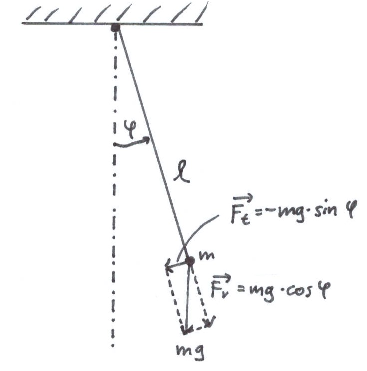
\includegraphics[scale=0.75]{Obrazky/Kyvadlo.pdf}
			\caption{Schéma jednoduchého kyvadla}
			\label{schema kyvadla}
		\end{wrapfigure}
		\begin{wrapfigure}{r}{0pt}
			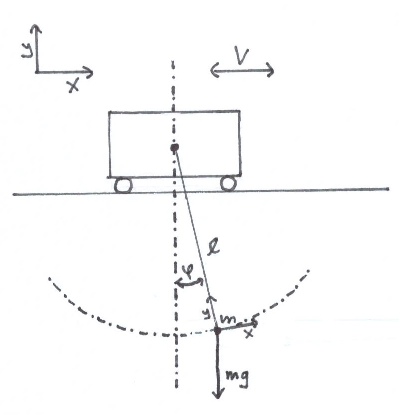
\includegraphics[scale=0.75]{Obrazky/Vozik-kyvadlo.pdf}
			\caption{Schéma soustavy vozík-kyvadlo}
			\label{schema vozik-kyvadlo}
		\end{wrapfigure}
		Pro potřeby návrhu tohoto modelu budeme uvažovat lano závěsu jako dokonale nepružné, o stálé délce $l$ a nulové hmotnosti $m_l = \SI{0}{\kilogram}$. Úhel vychýlení závěsu od osy vozíku označíme jako $\varphi$. Vozík se může pohybovat po ose x rychlostí $v$. Jako těleso si představíme bezrozměrný hmotný bod o hmotnosti $m$.\\
		Pro jednoduché kyvadlo připevněné k nepohybujícímu se tělesu (obr. \ref{schema kyvadla}) platí pohybová rovnice:
		\begin{align*}
			\ddot{\varphi}+\frac{g}{l}\sin\varphi=0
		\end{align*}
		Po zavěšení jednoduchého kyvadla na vozík budeme muset ještě do modelu přidat dynamiku vozíku.
\end{document}